
\section{Controlled Investigation of Influencing Factors}
\label{sec:controlled}

We next investigate whether Neon's reported robustness
extends to conditions relevant to driving, and which
factors contribute to the variability observed in the
real-world benchmark. Our systematically designed
controlled dataset comprises 216 recordings (2.9\,h)
from six participants, including repeated measurements
across varying viewing geometries, illumination,
motion, and sessions. This allows us to distinguish
conditions under which gaze accuracy remains stable
from systematic changes that may benefit from correction.
Table~\ref{tab:factors} summarizes the findings, while
Fig.~\ref{fig:controlled} presents the principal effects.

\begin{table*}[t]
\centering
\caption{Controlled evaluation across driving-relevant
factors. Participant counts indicate the available
experimental coverage. Reported effects are significant
after Holm correction unless stated otherwise.}
\label{tab:factors}
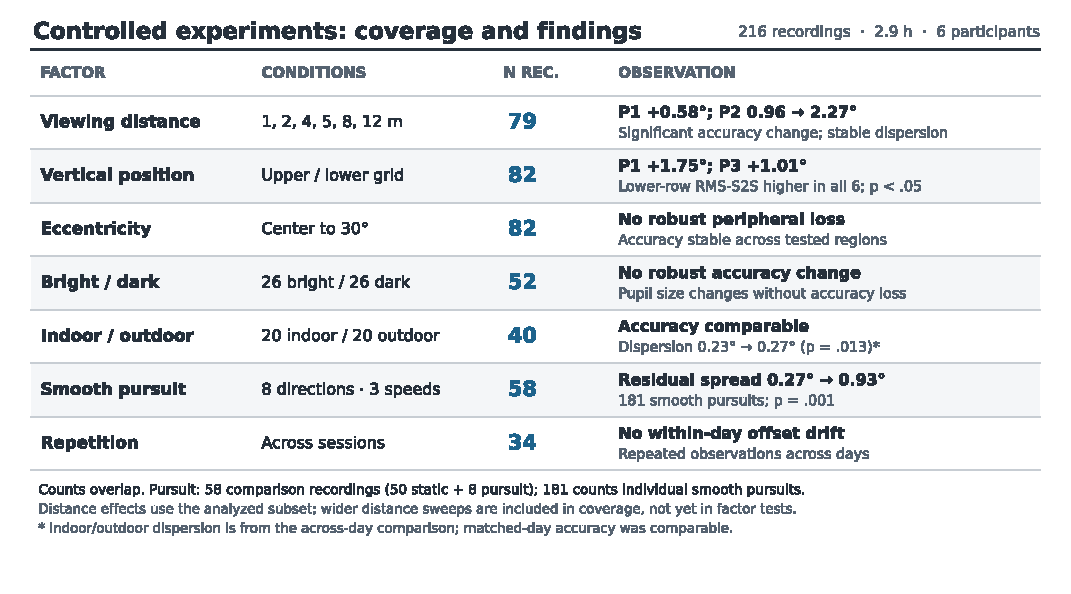
\includegraphics[width=\textwidth]
    {figures/tab_controlled_factors.pdf}
\end{table*}

\begin{figure*}[t]
\centering
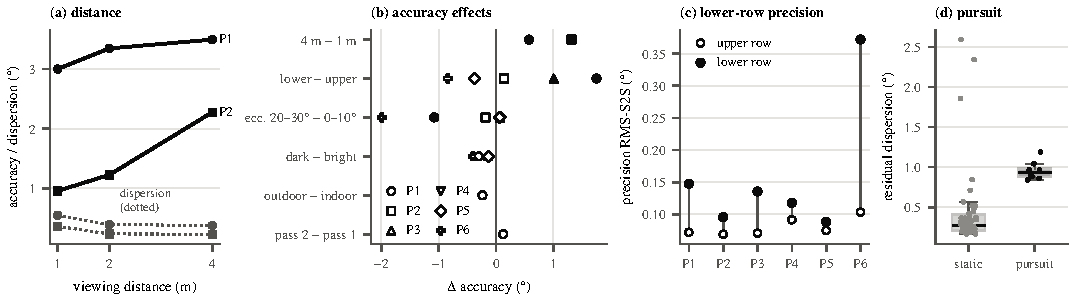
\includegraphics[width=\textwidth]
    {figures/fig3_controlled_factors.pdf}
\caption{Controlled evaluation of driving-relevant
influencing factors.
(a) Accuracy and dispersion versus viewing distance.
(b) Accuracy differences across experimental conditions;
filled markers indicate significant effects.
(c) Sample-to-sample precision in upper and lower
target rows.
(d) Residual dispersion during static fixation and
smooth pursuit.}
\label{fig:controlled}
\end{figure*}

\textbf{Robust accuracy across diverse conditions.}
A central finding is that Neon maintains largely stable
accuracy across several factors commonly encountered
during driving (Fig.~\ref{fig:controlled}b).
Despite changes in pupil diameter of 0.6--1.2\,mm
between bright and dark screen conditions, no
significant accuracy or dispersion differences were
detected. Similarly, matched indoor and outdoor
recordings yielded comparable accuracy (4.08\dg{}
and 3.85\dg{}, respectively), even as pupil diameter
decreased from 4.1 to 2.4\,mm outdoors. Only a small
increase in outdoor dispersion was observed
(0.23\dg{} to 0.27\dg{}, $p=.013$).

Accuracy also remained stable across gaze eccentricities
up to 30\dg{}, with no systematic deterioration towards
the image periphery among the five evaluated participants.
Repeated measurements showed no detectable within-day
drift over up to eight repetitions, and reversing the
fixation sequence did not significantly alter accuracy.
Together, these observations support the robustness
reported for Neon under varying illumination and gaze
conditions~\cite{baumann2026neonreport,salari2026pupilSize}.

\textbf{Viewing distance reveals systematic bias.}
Among the investigated factors, viewing distance
produced the clearest change in accuracy
(Fig.~\ref{fig:controlled}a). Across the evaluated
1, 2, and 4\,m conditions, median error increased
from 3.00\dg{} to 3.49\dg{} for P1 and from
0.96\dg{} to 2.27\dg{} for P2.
Both effects were significant (Holm $p<.001$ and
$p=.002$, respectively). The paired 1-to-4\,m
difference for P1 was 0.58\dg{}
(95\% CI [0.42, 0.75]).
Importantly, the change was primarily systematic:
gaze estimates shifted downwards with increasing
distance, while dispersion remained largely stable.
This suggests that the viewing geometry influences
the estimated gaze offset rather than introducing
additional measurement noise. The finding is
particularly relevant to driving, where targets
are often substantially farther away than
conventional calibration patterns, and offers
a possible explanation for the improved transfer
of driving-derived offsets in Sec.~\ref{sec:realworld}.

\textbf{Vertical gaze position affects measurement quality.}
Although radial eccentricity showed no general loss
of accuracy, the vertical position of the target
revealed a more specific spatial pattern.
At comparable eccentricities, lower-row targets
exhibited greater systematic error in two participants
(1.75\dg{} and 1.01\dg{} increases, both significant).
More consistently, sample-to-sample precision was
lower in the bottom row for all six participants
(Fig.~\ref{fig:controlled}c).
This distinction suggests that the spatial
distribution of gaze can influence both bias and
measurement stability, even when overall
peripheral accuracy remains robust.

\textbf{Smooth pursuit increases dispersion rather
than systematic error.}
Tracking moving targets is particularly relevant
to driving, where gaze frequently follows other
vehicles or traffic participants. In the evaluated
pursuit experiments, median accuracy and bias
remained comparable to static fixation.
However, target-relative dispersion increased
from 0.27\dg{} to 0.93\dg{}
(Holm $p=.001$; Fig.~\ref{fig:controlled}d).
Thus, dynamic gaze tracking primarily increased
the spread of measurements without introducing
a detectable systematic shift in this experiment.
This distinction is important when assessing
whether gaze observations provide reliable
supervision for moving targets.

\textbf{Implications for real-world gaze supervision.}
Overall, the controlled results reinforce Neon's
robustness across a broad range of tested conditions.
At the same time, they identify specific,
driving-relevant effects: viewing distance can
alter systematic gaze bias, lower visual-field
positions can affect measurement stability, and
dynamic tracking can increase dispersion.
These findings motivate separating systematic
correction from temporal noise reduction and
evaluating both directly on held-out driving
scenes in the following section.
